\chapter{Chirality}\label{sec:background:Chirality}

\begin{itemize}
    \item Figures for states of elliptically polarised light, showing linear combination of orthogonal components.
    \item Chirality in nature
    \begin{itemize}
        \item ``Chirality is exhibited by any molecule whose mirror-image cannot be superimposed onto itself and is exhibited by almost all biochemically and many pharmaceutically important molecules. Amino acids on earth are almost all exclusively ``left-handed'' and sugars ``right-handed''. ''
        \item General overview, examples of chirality being pervasive in nature
        \item Specific section on chemistry and biological molecular systems, with ``pop'' examples
        \item Examples of the need to rigorously characterise chiral systems
        \item Introduce the idea of using light as a probe for structural chirality
    \end{itemize}
\end{itemize}

The general mathematical form of a monochromatic plane wave at a distance $z$ and time $t$, oscillating at a frequency $\omega$, is given by equation~\ref{eq:background:chirality:generalwave}. The wave is polarised in the $x-y$ plane, and propagates along the $z$ axis with a wavevector $k_z$. $\phi$ describes the relative phase shift between the orthogonal components of polarisation, oscillating in the $\mathbf{\hat{x}}$ and $\mathbf{\hat{y}}$ directions with amplitudes $E_x$ and $E_y$ respectively.
\begin{equation} \label{eq:background:chirality:generalwave}
    \mathbf{E}= E_x  \mathbf{\hat{x}} \cos(k_z z-\omega t) - E_y \mathbf{\hat{y}} \cos(k_z z-\omega t +\phi)
\end{equation}
Linear combinations of $E_x$ and $E_y$, as in equation~\ref{eq:background:chirality:generalwave}, with no phase shift ($\phi=0$) result in linearly polarised light, with a polarisation axis depending on the relative amplitudes of $E_x$ and $E_y$. Crucially, linear combinations of $E_x$ and $E_y$ with non-zero amplitudes and a non-zero phase shift $\phi$ will result in a wave with angular momentum: The direction of polarisation rotates about the axis of propagation, tracing a helical profile. The ellipticity of this wave depends on both the phase and amplitude of the orthogonal linear components $E_x$ and $E_y$. Circular polarisation is the special case of a $\pm \pi/2$ phase shift between $E_x$ and $E_y$ of equal amplitude. The sign of the phase shift determines the direction of the polarisation rotation, resulting in left- and right-circularly polarised light (CPL). In this work, right-circularly polarised (RCP) light is defined as a clockwise rotation of the polarisation vector \textit{from the point of view of the wave source}. Conversely, left-circularly polarised (LCP) light is defined as a counter-clockwise rotation of the polarisation vector in the same frame. The wave equations for left- and right-circularly polarised light in this convention are given by equation~\ref{eq:background:chirality:CPL}~\cite[\S 8.1.2]{Hecht2013}). 
\begin{equation} \label{eq:background:chirality:CPL}
    \begin{split}
        & \mathbf{E}_{RCP} = E_0 \left[ \mathbf{\hat{x}} \cos(k_z z-\omega t) + \mathbf{\hat{y}} \sin(k_z z-\omega t )\right]\\
        & \mathbf{E}_{LCP}= E_0 \left[ \mathbf{\hat{x}} \cos(k_z z-\omega t) - \mathbf{\hat{y}} \sin(k_z z-\omega t )\right]
    \end{split}
\end{equation}
Since left- and right-circular polarisation states are orthogonal, any arbitrary polarisation can also be represented by the linear combination of LCP and RCP waves. For example, linear polarisation can be represented as the linear combination of equal amplitude LCP and RCP waves $\mathbf{E}_{LCP}$ and $\mathbf{E}_{RCP}$. 

Outside of the special case of CPL, the polarisation is described as elliptical, since both the total field amplitude, and the direction of polarisation, can vary as the wave propagates, resulting in an elliptical profile. The orientation of the elliptical profile, the ellipticity of the profile, and the direction of polarisation rotation, all depend on both the amplitudes of $E_x$ and $E_y$, and the phase between them.
Experimentally, elliptical and circular polarisations of light are realised by making use of an anisotropic, birefringent medium: One which has different refractive indices in orthogonal axes. Anisotropy in the real part of refractive index means that components of light polarised along the orthogonal axes, known as the medium's fast and slow axes, propagate with different phase velocities and accumulate a relative phase shift during propagation. By designing the thickness of the material such that the accumulated phase shift is $2m\pi \pm \pi/2$ at the operating wavelength $\lambda$ (where $m$ is some integer), elliptically and circularly polarised light can be obtained. Such a device is known as a quarter-wave plate (QWP), as it induces a shift of $\lambda/4$ between orthogonal polarisation components. The orientation of the elliptical profile depends on the direction of the incident polarisation, and the ellipticity depends on the angle of the material's fast axis relative to the direction of incident polarisation (figure~\ref{fig:background:Chirality:QWP}). Similarly, the orientation of linear polarisation can be rotated (known as ``optical rotation'', OR) by making use of a half-wave plate (HWP), which induces a relative phase shift of $2m\pi \pm \pi$ between orthogonal polarisation components. The angle of optical rotation also depends on the angle of the material's fast axis relative to the direction of incident polarisation.
\begin{figure}[htb!]
    \centering
    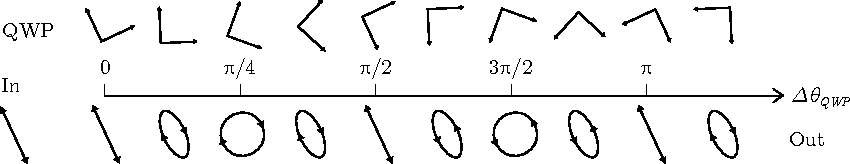
\includegraphics[scale=1.0]{./figures/background/chiroptics/QWP_in_out.pdf}
    \caption{\label{fig:background:Chirality:QWP}Output polarisation from a QWP at an angle $\Delta\theta_{QWP}$ to the input polarisation. The angle of the input (and subsequent elliptical and linear outputs) is controlled by the half-wave plate.}
\end{figure}

Whereas linear birefringence results from structural anisotropy, a medium with structural \textit{chirality}, such as a chiral molecular system, can exhibit a similar dissymmetry in it's interaction with LCP and RCP light. This leads to chiral-optical (chiroptical) effects, directly beneficial for polarisation optics, however also used to optically probe unknown properties of chiral structures. The rest of this chapter discusses the physical origin of chiroptical effects relevant to this work, and the parameters used to characterise the interactions between chiral structures and light.


\section{Structural Chirality}\label{sec:background:Chirality:Structural}
In the simple case of a linear, isotropic medium with no magnetoelectric coupling, the macroscopic electromagnetic response of the material is described by the constitutive relations given in equation~\ref{eq:background:chirality:isotropicConstitutive}. These relate the material's internal electric displacement field $\bf{\tilde D}$ and magnetic field strength $\bf{\tilde D}$ to the driving electric and magnetic fields $\bf{\tilde E}$ and $\bf{\tilde B}$. Here, $\varepsilon$ and $\mu$ are complex (denoted by a tilde) scalars and correspond to the isotropic electric permittivity and magnetic permeability of the material.
\begin{equation}\label{eq:background:chirality:isotropicConstitutive}
	\begin{split}
        & \bf{\tilde D} = \tilde \varepsilon \bf{\tilde E} \\
        & \bf{\tilde B} = \tilde \mu \bf{\tilde H}
	\end{split}
\end{equation}
In the general case however, we cannot assume isotropy and a lack of magnetoelectric coupling. For a bi-anisotropic medium, the constitutive relations take the form of equation~\ref{eq:background:chirality:fullConstitutive}.\cite{Ishimaru2003, Capolino2009}. Here, $\bf{\tilde \varepsilon}$, $\bf{\tilde \mu}$, $\bf{\tilde \xi}$, and $\bf{\tilde \zeta}$ are $3 \times 3$ matrices due to the anisotropy of the material. $\bf{\tilde \xi}$, and $\bf{\tilde \zeta}$ describe the magneto-electric cross-coupling.
\begin{equation}\label{eq:background:chirality:fullConstitutive}
    \begin{bmatrix}
        \bf{\tilde D} \\
        \bf{\tilde B}
    \end{bmatrix}
    =
    \begin{bmatrix}
        \bf{\tilde \varepsilon} & \bf{\tilde \xi} \\
        \bf{\tilde \zeta} & \bf{\tilde \mu}
    \end{bmatrix}
    \begin{bmatrix}
        \bf{\tilde E} \\
        \bf{\tilde H}
    \end{bmatrix}
\end{equation}
In the case of a non-gyrotropic material (exhibiting no magneto-optic rotation), equation~\ref{eq:background:chirality:fullConstitutive} has additional constraints, due to time-reversal symmetry, given in equation~\ref{eq:background:chirality:nongyroConstraints} \cite{Ishimaru2003}.
\begin{equation}\label{eq:background:chirality:nongyroConstraints}
    \begin{split}
        &[\bf{\tilde \xi}]^t = -[\bf{\tilde \zeta}] \\
        &[\bf{\tilde \varepsilon}]^t = [\bf{\tilde \varepsilon}] \\
        &[\bf{\tilde \mu}]^t = [\bf{\tilde \mu}]
    \end{split}
\end{equation}
The expressions shown in equation~\ref{eq:background:chirality:isotropicConstitutive} are a special case of equation~\ref{eq:background:chirality:fullConstitutive}, where no magneto-electric cross-coupling is present, so $\bf{\tilde \xi}=\bf{\tilde \zeta}=0$ and due to isotropy, $\bf{\tilde \varepsilon}$ and $\bf{\tilde \mu}$ become scalars. 
In the case of a non-chiral anisotropic material, $\bf{\tilde \xi}=\bf{\tilde \zeta}=0$ however $\bf{\tilde \varepsilon}$ and $\bf{\tilde \mu}$ remain as matrices. Most relevant in this discussion however is the special case of a bi-isotropic, or isotropic chiral, medium. 
In this case the matrix components reduce to scalars, but all four components remain. The constraints given in equation~\ref{eq:background:chirality:nongyroConstraints} apply, and so we find that $\xi =-\zeta $.

There are several ways to write the remaining relations, including Post's relations~\cite{Capolino2009}, Born's relations~\cite{Lekner1999, Barnett2016} , and Tellegen's relations~\cite{Capolino2009,kong1986,lindell1994} (equation~\ref{eq:background:chirality:tellegensRelations}). Tellegen's relations will be used here, however the various forms are equivalent.
\begin{equation}\label{eq:background:chirality:tellegensRelations}
    \begin{bmatrix}
        \mathbf{D} \\
        \mathbf{B}
    \end{bmatrix}
    =
    \begin{bmatrix}
        \varepsilon_0 \varepsilon_r & i \kappa \sqrt{\mu_0 \varepsilon_0} \\
        -i \kappa \sqrt{\mu_0 \varepsilon_0} & \mu_0 \mu_r
    \end{bmatrix}
    \begin{bmatrix}
        \mathbf{E} \\
        \mathbf{H}
    \end{bmatrix}
\end{equation}
Here, ${{\varepsilon }_{r}}$ and $\mu_r$ are the relative permittivity and permeability of the material respectively, and $\kappa$ is known as the ``chirality parameter''. Solving Maxwell's equations for a monochromatic plane wave propagating in the $z$ direction through the medium described by equation~\ref{eq:background:chirality:tellegensRelations} results in two eigenwaves with wave numbers given by equation~\ref{eq:background:chirality:kpmKappa}~\cite{Wang2014a, Qiu2008}, where $k_0$ is the wave number in vacuum. In a chiral medium these eigenwaves of wave number ${{k}_{+}}$ and ${{k}_{-}}$ correspond to right and left circularly polarized light respectively.
\begin{equation}\label{eq:background:chirality:kpmKappa}
    {k_\pm } = {k_0}\left( {\sqrt {{\mu _r}{\varepsilon _r}}  \pm \kappa } \right)
\end{equation}
From this, the corresponding refractive indices for RCP and LCP light are given by equation~\ref{eq:background:chirality:npmKappa}~\cite{Capolino2009, Qiu2008, Valev2013b}. 
\begin{equation}\label{eq:background:chirality:npmKappa}
    {n_ \pm } = \sqrt {{\mu _r}{\varepsilon _r}}  \pm \kappa
\end{equation}

\section{Chiroptical Effects}\label{sec:background:Chirality:Chiroptics}
Any material with a non-zero chirality parameter $\kappa$ will necessarily exhibit chiroptical effects dependent on it's real and imaginary parts. As in section~\ref{sec:background:Chirality:Structural}, the real part of the refractive index of a medium $n$ describes the phase velocity of light propagating through the medium, and the imaginary part describes the absorption of light by the medium. From equation~\ref{eq:background:chirality:kpmKappa}, $\operatorname{Im}(\kappa)$ thus describes the differential \textit{absorption} of LCP and RCP light, known as circular dichroism (CD). 
\begin{figure}[htb!]
    \centering
    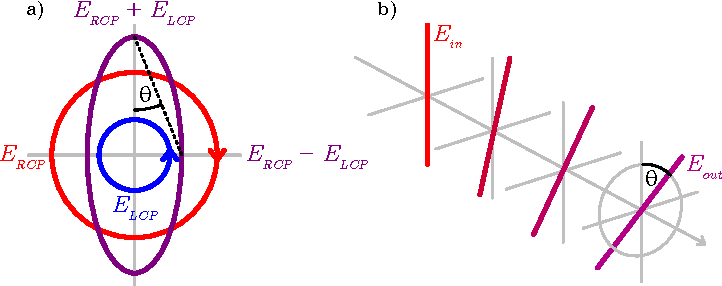
\includegraphics[scale=1.0]{./figures/background/chiroptics/cdor.pdf}
    \caption{\label{fig:background:Chirality:cdor}\textbf{a)} Schematic diagram of circular dichroism, characterised by the ellipticity ellipticity $\theta$ defined in terms of the field amplitudes of RCP and LCP light $E_{RCP}$ and $E_{LCP}$. The ellipticity is given by equation~\ref{eq:background:Chirality:CD}. \textbf{b)} Schematic diagram of optical rotation, showing linearly polarised light rotated by an angle $\theta$ throughout propagation through an optically active medium.}
\end{figure}
In linear optics, the circular dichroism at a particular wavelength of light is quantified by the ellipticity $\theta$, as defined by equation~\ref{eq:background:Chirality:CD}, and shown schematically in figure~\ref{fig:background:Chirality:cdor}a. 
\begin{equation}\label{eq:background:Chirality:CD}
    \theta = \arctan\left( \frac{E_{RCP} - E_{LCP}}{E_{RCP} + E_{LCP}} \right)
\end{equation} 
Here, $E_{RCP}$ and $E_{LCP}$ are the amplitudes of RCP and LCP light \textit{after} interaction with the chiral material. If $\operatorname{Im}(\kappa) = 0$, light can still be absorbed by the medium, but due to mirror symmetry, RCP and LCP light will emerge with equal amplitudes, and the CD as defined in equation~\ref{eq:background:Chirality:CD} is zero. For a non-zero $\operatorname{Im}(\kappa)$, $E_{RCP}$ and $E_{RCP}$ depend on both the magnitude of $\operatorname{Im}(\kappa)$, and the propagation length through the absorbing medium. If the propagation length is known, then circular dichroism can be used as a probe for the chirality parameter $\kappa$.
Correspondingly, $\operatorname{Re}(\kappa)$ describes the differential \textit{phase velocity} for LCP and RCP light. Since linearly polarised light can be represented by a superposition of equal-amplitude LCP and RCP waves, a linearly polarised wave, of vacuum wavevector $k_z$ propagating through a medium with RCP and LCP refractive indices given by $n_+$ and $n_-$ respectively, is described by equation~\ref{eq:background:Chirality:OR}~\cite[\S 8.10]{Hecht2013}.
\begin{equation}\label{eq:background:Chirality:OR}
    \begin{split}
        \mathbf{E} = E_0 \cos(k_z (\frac{n_+ + n_-}{2})z -\omega t &) \left[ \mathbf{\hat{x}} \cos(k_z (\frac{n_+ - n_-}{2})z ) \right. \\
        & \left. + \mathbf{\hat{y}} \sin(k_z (\frac{n_+ - n_-}{2}) z)\right]
    \end{split}
\end{equation}
At any point in time throughout propagation, the RCP and LCP components are oscillating in phase and with equal amplitudes, meaning that the resultant wave remains linearly polarised. However, the orientation of the linear polarisation will rotate throughout propagation, with the rate and direction of rotation depending on the magnitude and sign of $n_+ - n_-$ respectively. This effect is the chiral counterpart to birefringence, where orthogonal \textit{linear} polarisations exhibit different phase velocities. It is thus known as ``circular birefringence''. In the case of linear birefringence, optical rotation is achieved by utilising a fixed $\lambda/2$ phase shift, and rotating the mediums fast axis relative to the incident polarisation to control the angle of rotation. Conversely, a material exhibiting circular birefringence will rotate linearly polarised light continuously during propagation, shown schematically in figure~\ref{fig:background:Chirality:cdor}b. Therefore, the resulting angle of optical rotation ($\theta$ in figure~\ref{fig:background:Chirality:cdor}b) depends on both the strength of circular birefringence, and the propagation length through the medium. Optical rotation can therefore also be used as a method to characterise the chirality parameter $\kappa$ of the material. Collectively, circular dichroism and optical rotation are referred to as ``optical activity''.

Generally, in real materials the refractive index $n$ is strongly wavelength-dependent. This includes contributions from the structural chirality parameter, better given as $\kappa(\lambda)$. This directly leads to wavelength-dependent CD and OR, the latter specifically known as optical rotatory dispersion (ORD). CD spectra can be measured by taking extinction spectra LCP and RCP light propagating through the material, and applying equation~\ref{eq:background:Chirality:CD} at each wavelength, where $E_{RCP}$ and $E_{RCP}$ are the amplitudes of the transmitted RCP and LCP light respectively. Similarly, ORD spectra can be obtained by propagating linearly polarised light through the medium, and detecting the intensity of transmitted light through a rotatable analysing polariser. The analyser angle transmitting maximum intensity gives the resulting angle of polarisation, which can be compared to the incident polarisation to find the angle of optical rotation. Again, this can be taken at each wavelength to construct an ORD spectrum. It is important to reiterate however, that OR and CD depend on the real and imaginary parts of the same complex refractive index $n$. CD and ORD spectra are thus intrinsically linked by the Kramers-Kronig transforms: each can be obtained from the other, and they fundamentally contain the same information. 

\begin{itemize}
    \item Examples of chiral molecular geometries leading to CD and OR. Possibly discuss effects such as exciton-coupled CD in molecules? In the context of magneto-electric coupling, referring back to section~\ref{sec:background:Chirality:Structural}.
    \item References to papers and books discussing CD spectra and ORD as molecular characterisation techniques.
\end{itemize}



\subsection{Chiroptical Effects from Extrinsic Chirality}\label{sec:background:Chirality:extrinsic}
\begin{itemize}
    \item Lift some literature review content from my section in~\cite{Collins2017}.
\end{itemize}

It is possible to obtain a chiroptical response in plasmonic nanostructures that exhibit neither 3D nor planar chirality. Instead, chirality is introduced by the geometry of the experiment itself; the wave-vector, the surface normal and the direction of curvature on the sample form a chiral triad. 
The fundamental mechanism for this optical activity is shown in figure~\ref{fig:background:Chirality:extrinsic}. When illuminated at normal incidence, the structure geometry remains unchanged when projected onto the transverse plane of the incident light (figure~\ref{fig:background:Chirality:extrinsic} left). However, when the sample is illuminated at an oblique angle the projection of the structure geometry onto the transverse plane of incident light becomes distorted. Under inversion, the structure's projection can no longer be superimposed onto itself, and is therefore chiral, as shown in figure~\ref{fig:background:Chirality:extrinsic} right. Plum et al. showed that asymmetric transmission (circular difference) can occur in any array of nanostructures whose projection onto the transverse plane of incident light is 2-dimensionally chiral and anisotropic~\cite{Plum2011}. It is therefore possible to achieve chiroptical effects utilizing simpler structures than those that are intrinsically chiral; the latter being limited by the fabrication complexity. 
\begin{figure}[htb!]
    \centering
    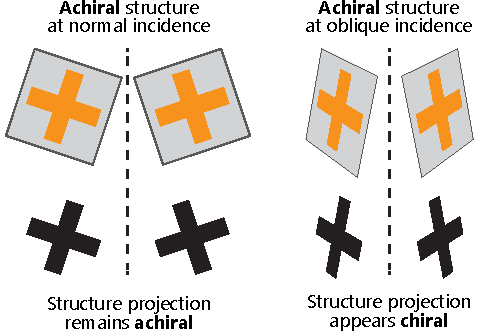
\includegraphics[scale=1.0]{./figures/background/chiroptics/extrinsic_chirality.pdf}
    \caption{\label{fig:background:Chirality:extrinsic}Schematic representation of extrinsic chirality in an achiral structure.}
\end{figure}

For applications requiring manipulation of light polarization, such as optical rotation or circular dichroism, it is perfectly possible to use extrinsic instead of intrinsic chirality. The relative simplicity of fabrication for achiral nanostructures could open the field to more readily available and easier to mass-produce geometries. The key here would be to consider the experimental geometry as a whole. However, in experiments aiming to characterise the chirality of materials at oblique incidence, contributions to measurable chiroptical effects from extrinsic chirality can serve to complicate analysis. Importantly, extrinsic chirality can be identified by considering the symmetry of the chiroptical response. If optical activity due to extrinsic chirality is measured at an oblique angle of incidence $\phi$, then the chiroptical response should change sign when measured at an angle of incidence of $-\phi$. That is, any measured circular dichroism will reverse sign, and any optical rotation will rotate in the opposite direction. This can perhpas be more intuitively understood by considering the geometry shown in figure~\ref{fig:background:Chirality:extrinsic}. The projection of the structure's mirror image at oblique incidence is identical it's own projection at the opposite angle of incidence. By reversing the angle of incidence, the chirality of the experimental geometry is reversed, and any chiroptical effects will correspondingly change sign.



\subsection{Chiroptical Effects from Anisotropy}\label{sec:background:Chirality:anisotropy}

\begin{itemize}
    \item Add some literature review content
\end{itemize}

It was shown earlier in section~\ref{sec:background:Chirality} that both optical rotation and the formation of circularly polarised light can occur in achiral materials due to only anisotropy. 
While the applications of this are clear, a potential issue is raised when characterising chiral systems. 
Within stereochemistry, chiroptical analysis historically tends to occur in isotropic, homogenous liquid molecular systems~\cite{Berova2012a}. In these cases, the anisotropy of individual molecules has no significant effect on the macroscopically measured optical activity. This is due to the 3-dimensional averaging out of anisotropy for a large number of randomly oriented molecules. 
However, this work makes frequent use of planar metallic ``nanomaterials'', discussed in greater depth in section~\ref{sec:background:Plasmonics}. These nano materials are commonly fabricated by patterning metallic inclusions onto a 2-dimensional surface, and so typically cannot be isotropically arranged. While some anisotropic symmetries can optically behave as though they are isotropic under certain experimental conditions (see section~\ref{sec:background:NonlinearOptics:rotation}), this is very much dependent on the geometry of illumination, and the out-of-plane depth of the nanostructure inclusions.

Much like for extrinsic chirality, chiroptical contributions from anisotropy can be identified with symmetry considerations. Any chiroptical effects measured due to an isotropic structure's intrinsic chirality will be invariant under structure rotation. Conversely, chiroptical effects originating exclusively from anisotropy will necessarily vary as the structure is rotated, reversing sign upon $\SI{90}{\degree}$ rotation normal to the fast and slow axis of the material. However, this periodic sign change is not strictly necessary in structures that exhibit both intrinsic chirality \textit{and} structural anisotropy. In these cases, the two contributions are effectively competing, and complex chiroptical behaviour can emerge~\cite{Hooper2017}. Isolating the structural chirality from anisotropy and extrinsic chirality is therefore challenging, especially in planar nanomaterials. In sections~\ref{sec:results:OAinPlanarNanohelices} and~\ref{sec:results:HRS} two methods of experimentally isolating the intrinsic chirality of metallic nanomaterials are explored.



\section{Optical Chirality and ``Superchiral'' Light}\label{sec:background:Chirality:opticalchirality}
The interaction between a chiral molecule and a chiral electromagnetic field is expected to exhibit a dissymmetry, in that each ``handedness'' of a chiral field should interact differently with a chiral molecule or nanostructure. A field with a shorter chiral pitch in the local EM field will exhibit a stronger interaction dissymmetry than a less twisted field. It had long been thought that the maximum possible chiral dissymmetry is obtained for a perfectly circularly polarized monochromatic field, however in 2010 Tang and Cohen proposed a setup in which the dissymmetry exceeds that of CPL (referred to as ``superchiral light'') at the nodes of a chiral standing wave.~\cite{Tang2010}
The strength of the field chirality can be quantified by Lipkin's 00-zilch density~\cite{Lipkin1964} referred to by Tang and Cohen as the ``optical chirality'' $C$ as given in equation~\ref{eq:background:chirality:opticalchirality}.
\begin{equation} \label{eq:background:chirality:opticalchirality}
    \begin{split}
        C = &\frac{\varepsilon_0 }{2}{\bf{\tilde E}} \cdot (\nabla  \times {\bf{\tilde E}}) + \frac{1}{{2\mu _0}}{\bf{\tilde B}} \cdot (\nabla  \times {\bf{\tilde B}}) \\
        = &- \frac{{{\varepsilon _0}\omega }}{2} \operatorname{Im}[ \bf{\tilde E}(\bf{r}) \cdot \bf{\tilde B}(\bf{r}) ]
    \end{split}
\end{equation}
Here, $\bf{\tilde E}$ and $\bf{\tilde B}$ denote the complex electric and magnetic field amplitudes respectively. This quantity describes the angular momentum of the curl of the optical field~\cite{Cameron2012a} and is a conserved property of the field. Tang and Cohen showed that the enantioselectivity of optical excitation of a molecule is highly dependent on $C$, and so it stands that such a superchiral field can lead to significant enhancement of the enantioselective excitation of chiral molecules.

The general response of a chiral molecule to a monochromatic electromagnetic field is described by an internal electric dipole moment $\mathbf{\tilde p}$ and magnetic dipole moment $\mathbf{\tilde m}$ as in equation~\ref{eq:background:chirality:tangDipole}.
\begin{equation}
    \label{eq:background:chirality:tangDipole}
    \begin{split}
        &{\bf{\tilde p}} = {{\tilde \alpha }_{ee}}{\bf{\tilde E}} - i{{\tilde \alpha }_{em}}{\bf{\tilde B}} \\
        &{\bf{\tilde m}} = i{{\tilde \alpha }_{em}}{\bf{\tilde E}} + {{\tilde \alpha }_{mm}}{\bf{\tilde B}}
    \end{split}
\end{equation}
Here, $\tilde{\alpha}_{ee}$ and $\tilde{\alpha}_{mm}$ correspond to $\tilde{\alpha}$ and $\tilde{\chi}$ in references~\cite{Tang2010} and~\cite{Choi2012}, 
$\alpha_{ee}$ is the electric polarisability, and $\alpha_{mm}$ is the magnetic susceptibility. $\tilde{\alpha}_{em}$ is the mixed magneto-electric polarisability and is directly related to the material chirality parameter $\kappa$ (section~\ref{sec:background:Chirality:Structural}).
Physical quantities are obtained from the real parts of equation (14). For an incident $\mathbf{\tilde{E}}=\mathbf{\tilde{E}}_{0}{e}^{-i\omega t}$ and $\mathbf{\tilde{B}}=\mathbf{\tilde{B}}_{0}{e}^{-i\omega t}$ the rate of excitation of a molecule from right ($+$) and left ($-$) CPL is given by equation~\ref{eq:background:chirality:Aplusminus} \cite{Tang2010, Choi2012}.

\begin{equation} \label{eq:background:chirality:Aplusminus}
    {A^ \pm } = 
    \frac{\omega }{2}{\left\langle {{\bf{E}} \cdot {\bf{\dot p}} + {\bf{B}} \cdot {\bf{\dot m}}} \right\rangle _t} = 
    \frac{\omega }{2}{\mathop{\rm Im}\nolimits} ({{\bf{\tilde E}}^ * } \cdot {\bf{\tilde p}} + {{\bf{\tilde B}}^ * } \cdot {\bf{\tilde m}})
\end{equation}
Substituting equation~\ref{eq:background:chirality:tangDipole} into equation~\ref{eq:background:chirality:Aplusminus} leads to equation~\ref{eq:background:chirality:AplusminusFull}, which can be rewritten in terms of the generalized optical chirality $C$ to give equation~\ref{eq:background:chirality:AplusminusC}~\cite{Choi2012}. Here ${\tilde \alpha }_{em}''=\operatorname{Im}({\tilde \alpha }_{em})$.
\begin{equation} \label{eq:background:chirality:AplusminusFull}
    {A^ \pm } = \frac{\omega }{2}({\tilde \alpha ''_{ee}}{\left| {{\bf{\tilde E}}} \right|^2} + {\tilde \alpha ''_{mm}}{\left| {{\bf{\tilde B}}} \right|^2}) \pm {\tilde \alpha }_{em}''\omega {\mathop{\rm Im}\nolimits} ({{\bf{\tilde E}}^ * } \cdot {\bf{\tilde B}})
\end{equation}
\begin{equation} \label{eq:background:chirality:AplusminusC}
    {A^ \pm } \simeq \frac{\omega }{2}({\tilde \alpha ''_{ee}}{\left| {{\bf{\tilde E}}} \right|^2} + {\tilde \alpha ''_{mm}}{\left| {{\bf{\tilde B}}} \right|^2}) \pm {\tilde \alpha }_{em}''\frac{2}{\varepsilon }C
\end{equation}
The time averaged electric and magnetic energy densities ${{\left\langle {{U}_{E}} \right\rangle }_{t}}=\tfrac{\varepsilon }{4}{{\left| {\mathbf{\tilde{E}}} \right|}^{2}}$ and ${{\left\langle {{U}_{B}} \right\rangle }_{t}}=\tfrac{1}{4\mu }{{\left| {\mathbf{\tilde{B}}} \right|}^{2}}$  can be introduced here, and substituted into equation~\ref{eq:background:chirality:AplusminusC} to give the rate of excitation in terms of energy density as in equation~\ref{eq:background:chirality:AplusminusU}. 
\begin{equation}\label{eq:background:chirality:AplusminusU}
    \begin{split}
        & {A^ \pm } \simeq \frac{2}{\varepsilon }{{\tilde \alpha ''}_{ee}}\omega \left( {{{\left\langle {{U_E}} \right\rangle }_t} + \gamma {{\left\langle {{U_B}} \right\rangle }_t}} \right) \pm {\tilde \alpha }_{em}''\frac{2}{\varepsilon }C \\
        & \gamma  = \frac{{{{\tilde \alpha ''}_{mm}}}}{{{{\tilde \alpha ''}_{ee}}}}\varepsilon \mu  = \frac{{{{\tilde \alpha ''}_{mm}}}}{{{{\tilde \alpha ''}_{ee}}}}\frac{{{n^2}}}{{{c^2}}}
    \end{split}
\end{equation}
We can now define the dissymmetry factor $g$ of the chiroptical interaction by equation~\ref{eq:background:chirality:dissymmetryA}.
\begin{equation}\label{eq:background:chirality:dissymmetryA}
    g = \frac{{{A^ + } - {A^ - }}}{\frac{1}{2}({A^ + } + {A^ - })}
\end{equation}
In Tang and Cohen's proposal~\cite{Tang2010} the magnetic field was disregarded as negligible. Under this assumption, the dissymmetry factor is found to be 
\begin{equation}\label{eq:background:chirality:dissymmetryG}
    g =  - \frac{{{\tilde \alpha }_{em}''}}{{\tilde \alpha ''}_{ee}}\frac{{2C}}{{\omega {{\left\langle {{U_E}} \right\rangle }_t}}}
\end{equation}
Note that under this approximation, the dissymmetry factor splits into properties of the molecule only (${{\tilde \alpha }_{em}''}/{{\alpha }''}_{ee}$) and properties of the field only (${2C}/{\omega {{\left\langle {{U}_{E}} \right\rangle }_{t}}}$), however in the general case the dissymmetry factor cannot be separated in this way and is significantly more complex~\cite{Choi2012}.
The full expression accounting for magnetic energy density can be simplified by assuming a small dissymmetry factor such that $n_{LCP} \approx n_{RCP}$, to give equation~\ref{eq:background:chirality:dissymmetryFull}.~\cite{Choi2012}
\begin{equation}\label{eq:background:chirality:dissymmetryFull}
    g =  - \frac{{\tilde \alpha ''}_{em}}{{{\tilde \alpha ''}_{ee}}}\frac{{2C}}{{\omega [{{\left\langle {{U_E}} \right\rangle }_t} + \gamma {{\left\langle {{U_B}} \right\rangle }_t}]}}
\end{equation}
The limitation in chiroptical enhancement is now clear: at regions of low electric energy density, the magnetic energy density is maximized and should not be considered negligible. The $\gamma$ term in equation~\ref{eq:background:chirality:dissymmetryFull} is then the key limiting factor for the dissymmetry enhancement. The energy density terms in the denominator can no longer be reduced to arbitrarily small values in order to continually increase chiral dissymmetry. However, the chiral dissymmetry can still be increased by reducing the total electromagnetic energy density, increasing the structural chirality parameter of the medium, and increasing optical chirality $C$ of the electromagnetic field. 

\begin{itemize}
    \item Brief literature review of any papers discussing, or demonstrating, superchiral fields using standing waves (or generally anything that doesn't use plasmonic nanomaterials, as this is covered later in section~\ref{sec:background:Plasmonics:superchiral}).
\end{itemize}